\documentclass[14pt]{extarticle}

\usepackage{fontspec}
\setmainfont{Times New Roman}

% размер полей
\usepackage{geometry}
\geometry{a4paper, top=2cm, bottom=2cm, right=1.5cm, left=3cm}

 %debugging
%\usepackage{showframe}

% полуторный интервал
\usepackage{setspace}
\onehalfspacing

% абзацный отступ
\setlength{\parindent}{1.25cm}

% выравнивание текста по ширине
\sloppy

% списки
\usepackage{calc} % арифметические операции с величинами
\usepackage{enumitem}
\setlist{
    nosep,
    leftmargin=0pt,
    itemindent=\parindent + \labelwidth - \labelsep,
}

% подписи к рисункам и таблицам
\usepackage{caption}
\renewcommand{\figurename}{Рисунок}
\renewcommand{\tablename}{Таблица}
\DeclareCaptionFormat{custom}
{
    \textit{#1#2#3}
}
\DeclareCaptionLabelSeparator{custom}{. }
\captionsetup{
    % хз какой это размер - 12 или нет, но выглядит меньше 14
    font=small,
    format=custom,
    labelsep=custom,
}

% картинки
\usepackage{graphicx}

% колонтитулы
\usepackage{fancyhdr}

% картинки и таблицы находятся именно в том месте текста где помещены (атрибут H)
\usepackage{float}

% таблицы
\usepackage{tabularray}

\graphicspath{ {2.1/models/} }
\usepackage{hyperref}
\usepackage{upgreek}
\begin{document}
\pagestyle{fancy}
\fancyhead{}
% disable header
\renewcommand{\headrulewidth}{0pt}
\singlespacing

\newpage
\begin{center}
    Министерство науки и высшего образования Российской Федерации
    Федеральное государственное автономное образовательное учреждение

    высшего образования

    \guillemotleft МОСКОВСКИЙ ПОЛИТЕХНИЧЕСКИЙ УНИВЕРСИТЕТ\guillemotright

    (МОСКОВСКИЙ ПОЛИТЕХ)
\end{center}
\noindent
\bigbreak
\bigbreak
\bigbreak
\bigbreak
\begin{center}
    \textbf{ОСНОВНЫЕ ПОНЯТИЯ, ТЕРМИНЫ И РАСПРЕДЕЛЕНИЯ ИЗ
ТЕОРИИ ВЕРОЯТНОСТЕЙ}
    \bigskip
    \bigskip
    \bigskip
    \bigskip
    \bigskip

    Лабораторная работа 2.1

    По курсу \guillemotleft Надёжность информационных систем\guillemotright
    \bigskip

    \bigbreak
    \bigbreak
    \bigbreak
    \bigbreak
\end{center}
\noindent
\bigbreak
\bigbreak
\bigbreak
\bigbreak
\bigbreak
\bigbreak
\bigbreak
\bigbreak
\bigbreak
\bigbreak
\hfill Выполнил

\hfill Дубровских Н.Е.

\hfill Группа 221-361
\bigbreak
\bigbreak
\bigbreak
\hfill Проверил

\hfill Маковей С.О.
\vfill
\begin{center}
    Москва, 2024
\end{center}
\newpage
\onehalfspacing


\begin{center}
    \textbf{Лабораторная работа 2.1}

    \textbf{Основные распределения, используемые в
теории надежности. Распределение Бернулли. Геометрическое
распределение. Экспоненциальное распределение.
Гиперэкспоненциальное распределение. Биномиальное распределение.}
\end{center}

К \textbf{основным целям} лабораторной работы следует отнести:

\begin{itemize}
    \item формирование у студентов понимания важности развития и применения средств теории вероятностей в современных информационных системах и технологиях;
    \item ознакомление студентов с основными распределениями теории вероятностей.
\end{itemize}

К \textbf{основным задачам} лабораторной работы следует отнести:

\begin{itemize}
    \item анализа состояния и тенденций развития теории вероятностей;
    \item развитие навыков изучения истории и областей применения методов теории вероятностей;
    \item развитие навыков классификации средств теории вероятностей.
\end{itemize}
\bigskip

\pagebreak

\begin{center}
\textbf{ОТЧЁТ ПО ВЫПОЛНЕНИЮ}
\end{center}

\textbf{Задача № 1}

Инициализируется тестовая DDoS-атака на сервер, где действует комплексная
система защиты. Среднее время работы сервера до отказа равно $T_0$ = 20000ч.
Справедлив экспоненциальный закон надёжности. Определить вероятность
безотказной работы сервера в течение времени 16000 час, частоту отказов для
момента времени 10000 час.

Определяем интенсивность отказов

$ \lambda (20000) = 1 / T_0 = 1 / 20000 = 0.00005$ 1/ч

Определяем вероятность безотказной работы сервера в течении времени 16000 час

$P(16000) = e^{-\lambda t} = e^{-0.00005 \cdot 16000} = 0.44932896411722156 \approx 44.93\%$

Определяем частоту отказов для момента времени 10000 час

$f(10000) = \lambda e^{-\lambda t} = 0.00005e^{-0.00005 \cdot 10000} = 0.00003032653298563167 \approx 0.0000303$ 1/ч

\bigskip

\textbf{Задача 2.}

Усилитель низкой частоты собран на элементной базе
радиокомпонентов. Состав элементов усилителя сведён в таблицу.
Условия эксплуатации характеризуются коэффициентом нагрузки $K_H$ =
0.5, температурой $T^0$ = $40^0$С. Требуется определить основные
количественные показатели надёжности за время работы t = 720 час, t =
8760 час.

\noindent
\begin{minipage}[H]{\linewidth}
    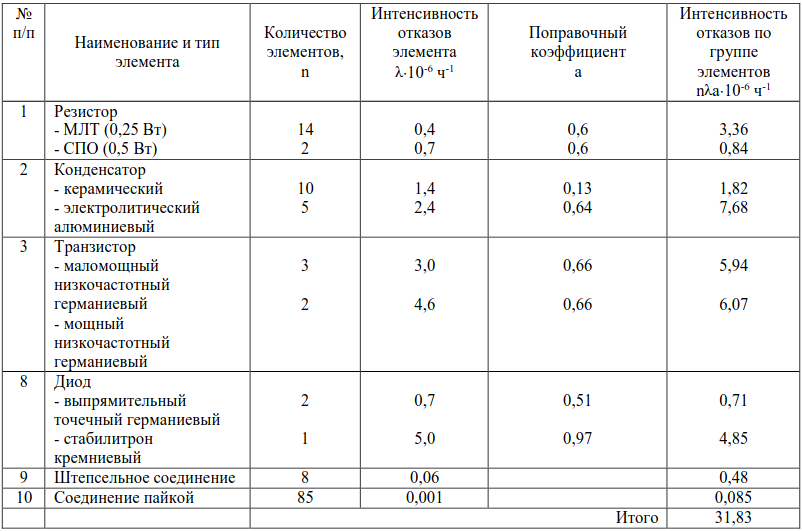
\includegraphics[width=\linewidth]{table}
\end{minipage}
\bigskip

Интенсивность отказов

$\lambda = 31.83 \cdot 10^{-6}$

Определим вероятность безотказной работы

$P(720) = e^{-\lambda t} = e^{-31.83 \cdot 10^{-6} \cdot 720} = 0.97734301351972 \approx 97.73\%$

$P(8760) = e^{-\lambda t} = e^{-31.83 \cdot 10^{-6} \cdot 8760} = 0.7566679205966365 \approx 75.58\%$

Определим вероятность отказа

$Q(720) = 1 - P(720) = 1 - 0.97734301351972 = 0.022656986480280028 \approx 2.27\%$

$Q(8760) = 1 - P(8760) = 1 - 0.7566679205966365 = 0.24333207940336354 \approx 24.42\%$

Определим наработку до отказа

$T_0 = \frac{1}{\lambda} = \frac{1}{31.83 \cdot 10^{-6}} = 31416.902293433868$ ч. $ = 3.58640437139656$ лет
$\approx 3.6 $ лет

\end{document}
